% Compilar a .pdf con LaTeX (pdflatex)
% Es necesario instalar Beamer 
%

\documentclass{beamer}
\usepackage{moreverb} 
\usepackage{listings}
\usepackage{mflogo}
% imprimir
% \documentclass[handout]{beamer} 
% \usepackage{pgfpages}
% \pgfpagesuselayout{4 on 1}[a4paper,landscape,border shrink=5mm]

\mode<presentation> {
  \usetheme{Warsaw}
  \setbeamercovered{transparent}
}

\usebackgroundtemplate{
\includegraphics[width=\paperwidth]{format/libresoft-bg.png}}
\usepackage[spanish]{babel}
\usepackage[utf8]{inputenc}
\usepackage{graphics}
\usepackage{amssymb} % Simbolos matematicos

%% Metadatos del PDF.
\hypersetup{  
  pdftitle={Historia del software libre},
  pdfauthor={Miguel Vidal},
  pdfcreator={GSyC/Libresoft},
  pdfproducer=PDFLaTeX,
  pdfsubject={Master on Free Software},
}
%%

\setbeamercovered{invisible} % evita que se vea en el /pause
\defbeamertemplate*{footline}{shadow theme}
{%
  \leavevmode%
  \hbox{\begin{beamercolorbox}[wd=.5\paperwidth,ht=2.5ex,dp=1.125ex,leftskip=.3cm plus1fil,rightskip=.3cm]{author in head/foot}%
    \usebeamerfont{author in head/foot}\insertframenumber\,/\,\inserttotalframenumber\hfill
\includegraphics[scale=0.40]{format/cc-by-80x15.png} \hspace{0.1cm}\insertshortauthor 
% \usebeamerfont{author in head/foot} 
\includegraphics[width=0.7cm]{format/cc-by.png} \hfill\insertshortauthor
  \end{beamercolorbox}%
  \begin{beamercolorbox}[wd=.5\paperwidth,ht=2.5ex,dp=1.125ex,leftskip=.3cm,rightskip=.3cm plus1fil]{title in head/foot}%
    \usebeamerfont{title in head/foot}\insertshorttitle%
  \end{beamercolorbox}}%
  \vskip0pt%
}

\begin{document}

\title{Historia del software libre}
\subtitle{Master on Free Software (URJC)}
\institute{\texttt{http://gsyc.urjc.es/\~{}mvidal} \\ Twitter: \texttt{@mvidallopez}}
\author{Miguel Vidal} 
%\date{\today}
\date{November, 2011}

\frame{
\maketitle
\begin{center}

\includegraphics[width=6cm]{format/gsyc-urjc}
\end{center}
}

%% License slide
\begin{frame}
  \vspace{2cm}
  \begin{flushright}
    {\small \copyright{} 2008-2011 Miguel Vidal, Jesús González Barahona} \\
%    \vspace{0.25cm}
    \medskip
    {\scriptsize This work is licensed under \\ a Creative Commons Attribution 3.0 License}
%    \vspace{0.10cm}
  \end{flushright}
  \begin{flushright}
    \href{http://creativecommons.org/licenses/by/3.0/es}{
\includegraphics[width=2cm]{format/cc-by.png}} \\
    {\tiny \url{http://creativecommons.org/licenses/by/3.0}}
  \end{flushright}
\end{frame}%%

\usebackgroundtemplate{}

\AtBeginSection[]
{
\begin{frame}<beamer>
\begin{center}
{\LARGE \insertsection}
\end{center}
\end{frame}
}


\AtBeginSubsection[]
{
  \begin{frame}<beamer>{Table of Contents}
    \tableofcontents[currentsection,currentsubsection]
  \end{frame}
}


%%%%%%%%%%%%%%%%%%%%%%%%%%%%%%%%%%%%%%%%%%%%%%%%%%%%%%%%%%%%%%%%%%%%%%%
\section{Historia del software libre}
%%%%%%%%%%%%%%%%%%%%%%%%%%%%%%%%%%%%%%%%%%%%%%%%%%%%%%%%%%%%%%%%%%%%%%%


\begin{frame}
\frametitle{Historia del software libre}

\begin{itemize}

\item {Se remonta a los orígenes de la informática.}
\item {Como movimiento consciente, nace en 1984 con el Proyecto GNU.}
\item {En los 90, Linux y el modelo bazar suponen su culminación.}

\end{itemize}

\end{frame}

%%%%%%%%%%%%%%%%%%%%%%%%%%%%%%%%%%%%%%%%%%%%%%%%%%%%%%%%%%%%%%%%%%%%%%%


\begin{frame}
\frametitle{Orígenes: ``Real Programmers''}

\begin{itemize}

\item 1945 hasta 1970: los \textit{Real Programmers} fueron la cultura técnica dominante en el ámbito de la computación. 
\item Desde el primer computador ENIAC, existió una cultura técnica, consciente de sí misma, creaban y manipulaban software por pura diversión. 
\item Los \textit{Real Programmers} eran ingenieros o físicos, y a menudo radioaficionados. 
\item Seymour Cray, diseñador de la gama de supercomputadoras Cray, fue uno de los más brillantes.
\item Son los pioneros de la informática actual.

\end{itemize}

\end{frame}

%%%%%%%%%%%%%%%%%%%%%%%%%%%%%%%%%%%%%%%%%%%%%%%%%%%%%%%%%%%%%%%%%%%%%%%

\begin{frame}
\frametitle{Un ``Real Programmer'': Seymour Cray}


\begin{figure}[h]

\begin{center}
  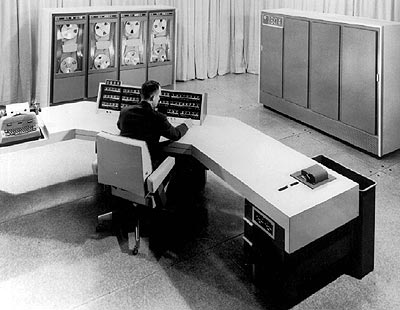
\includegraphics[height=1.80in]{figs/cray_sm.jpg}
  \caption{{\footnotesize Seymour Cray, con un supercomputador CDC 1604 diseñado por él, en 1958}}
\end{center}
\end{figure}


\end{frame}


%%%%%%%%%%%%%%%%%%%%%%%%%%%%%%%%%%%%%%%%%%%%%%%%%%%%%%%%%%%%%%%%%%%%%%%


\begin{frame}
\frametitle{Las décadas de 1950 y 1960}

\begin{itemize}

\item Durante los años 1960 el software venía como acompañante del hardware, no se considera un elemento independiente.
\item El software se distribuía con su código fuente: grupos de usuarios lo comparten, y lo mejoran.
\item Código fuente a disposición de quien lo pide: los clientes generalmente no pagan por el software. 
\item Relación con el software muy parecida a la que hoy tenemos con el software libre.
\item Todo cambia con el \textit{unbundling} de hardware, software y servicios de IBM (1969)
\end{itemize}

\end{frame}



%%%%%%%%%%%%%%%%%%%%%%%%%%%%%%%%%%%%%%%%%%%%%%%%%%%%%%%%%%%%%%%%%%%%%%%


\begin{frame}
\frametitle{Los primeros hackers}

\begin{itemize}

\item 1961: el MIT adquiere la primera PDP-1. La usa el Tech Model Railroad Club (TMRC), núcleo del IA Lab del MIT. 
\item La cultura en torno a las computadoras del MIT adopta el término ``hacker'' y crean su propio SO para PDP-10 (ITS, ``Incompatible Timesharing System'', sin permisos ni contraseñas).
\item Allí se forma Stallman, y surge la cultura de Arpanet (\textit{jargon file}).
\item ARPANET (principalmente una red de computadoras DEC) interconecta a hackers de toda Norteamérica y es la génesis de Internet.
\item Otro nodo importante: el PARC de XEROX, en Palo Alto (California). 

\end{itemize}

\end{frame}

%%%%%%%%%%%%%%%%%%%%%%%%%%%%%%%%%%%%%%%%%%%%%%%%%%%%%%%%%%%%%%%%%%%%%%%


\begin{frame}
\frametitle{¿Hackers?}

¿Piratas informáticos?

\pause

\begin{block}{Definición original de hacker}
\footnotesize{``Existe una comunidad, una cultura compartida, de programadores expertos y genios de las redes, cuya historia se remonta décadas atrás a los tiempos de los primeros miniordenadores de tiempo compartido y los tempranos experimentos con ARPAnet. Los miembros de esta cultura crearon el término ``hacker''. Los hackers construyeron Internet. Los hackers hicieron de Unix el sistema operativo que es hoy día. Los hackers hacen andar Usenet. Los hackers hacen funcionar la WWW. Si eres parte de esta cultura, si has contribuido a ella y otras personas saben quién eres y te llaman hacker, entonces eres un hacker.'' (\textsc{Eric Raymond})}
\end{block}

\end{frame}


%%%%%%%%%%%%%%%%%%%%%%%%%%%%%%%%%%%%%%%%%%%%%%%%%%%%%%%%%%%%%%%%%%%%%%%

\begin{frame}
\frametitle{Ética hacker}

\begin{itemize}
\item {Un buen programador debería contribuir con su trabajo a la
comunidad}
\item {Un buen programador debería poder aprovechar el trabajo de otros
buenos programadores}
\item {Un buen programador debería poder ``arreglar'' y mejorar cualquier
programa}
\item {Un buen programador debería sentirse orgulloso de su propio
código y de que otros lo usen, sin otras contraprestaciones.}
\end{itemize}

\pause

\begin{center}
\alert{Buen programador == \textbf{hacker}}
\end{center}

\end{frame}


%%%%%%%%%%%%%%%%%%%%%%%%%%%%%%%%%%%%%%%%%%%%%%%%%%%%%%%%%%%%%%%%%%%%%%%

\begin{frame}
\frametitle{Años setenta}

\begin{itemize}

\item El software empieza a ser privativo ``por defecto''
\item Esfuerzos ``aislados'': TeX, Spice, etc.
\item En general, el objetivo es hacer una herramienta determinada
	\begin{itemize}
	\item A veces, motivos éticos (ej: costumbre en la comunidad matemática)
	\item A veces, motivos prácticos (ej: difusión de una nueva tecnología)
	\end{itemize}
\end{itemize}

\end{frame}


%%%%%%%%%%%%%%%%%%%%%%%%%%%%%%%%%%%%%%%%%%%%%%%%%%%%%%%%%%%%%%%%%%%%%%%

\begin{frame}
\frametitle{Años setenta: El surgimiento de Unix}

El nacimiento de Unix, una auténtica revolución del software:

\begin{itemize}

\item 1969: Ken Thompson inventó Unix (mismo año que Arpanet).
\item Surge de los deshechos de Multics, en AT\&T (Bell Labs). 
\item Dennis Ritchie inventa un nuevo lenguaje llamado C para usarlo en el Unix de Thompson. 
\item Primer sistema operativo portable y modular (KISS), frente a anteriores sistemas incompatibles y costosos.
\item Se extiende rápidamente y de forma no oficial por AT\&T. Y por Arpanet (hardware distinto, gracias a C).
\item Acuerdo judicial (\textit{antitrust}) de 1956 impide a AT\&T comercializar Unix: debe licenciarlo (con fuentes) a quien se lo solicite.

\end{itemize}

\end{frame}

%%%%%%%%%%%%%%%%%%%%%%%%%%%%%%%%%%%%%%%%%%%%%%%%%%%%%%%%%%%%%%%%%%%%%%%

\begin{frame}
\frametitle{Años setenta: Unix y Berkeley}

\begin{itemize}

\item CSRG (Computer Systems Research Group) de Berkeley:
	\begin{itemize}
	\item Importancia de compartir fuentes (cultura Unix ``original'').
	\item Limitado por la licencia AT\&T (poco desde el punto de vista práctico, todos la tenían).
	\item Financiado por DARPA (DoD).
	\item Utilizado por mucho software propietario (SunOS, Ultrix, etc.)
	\end{itemize}

\item Primera Internet:
	\begin{itemize}
	\item Implementaciones de referencia, disponibles para todos: la base de los estándares actuales.
	\item La Red como herramienta de cooperación (News, ftp, e-mail).
	\item La comunidad de usuarios proporciona el mejor soporte.
        \item Falso mito de los ataques nucleares. 
	\end{itemize}

\end{itemize}

\end{frame}

%%%%%%%%%%%%%%%%%%%%%%%%%%%%%%%%%%%%%%%%%%%%%%%%%%%%%%%%%%%%%%%%%%%%%%%

\begin{frame}
\frametitle{Historia de Unix}


\begin{figure}[h]

\begin{center}
  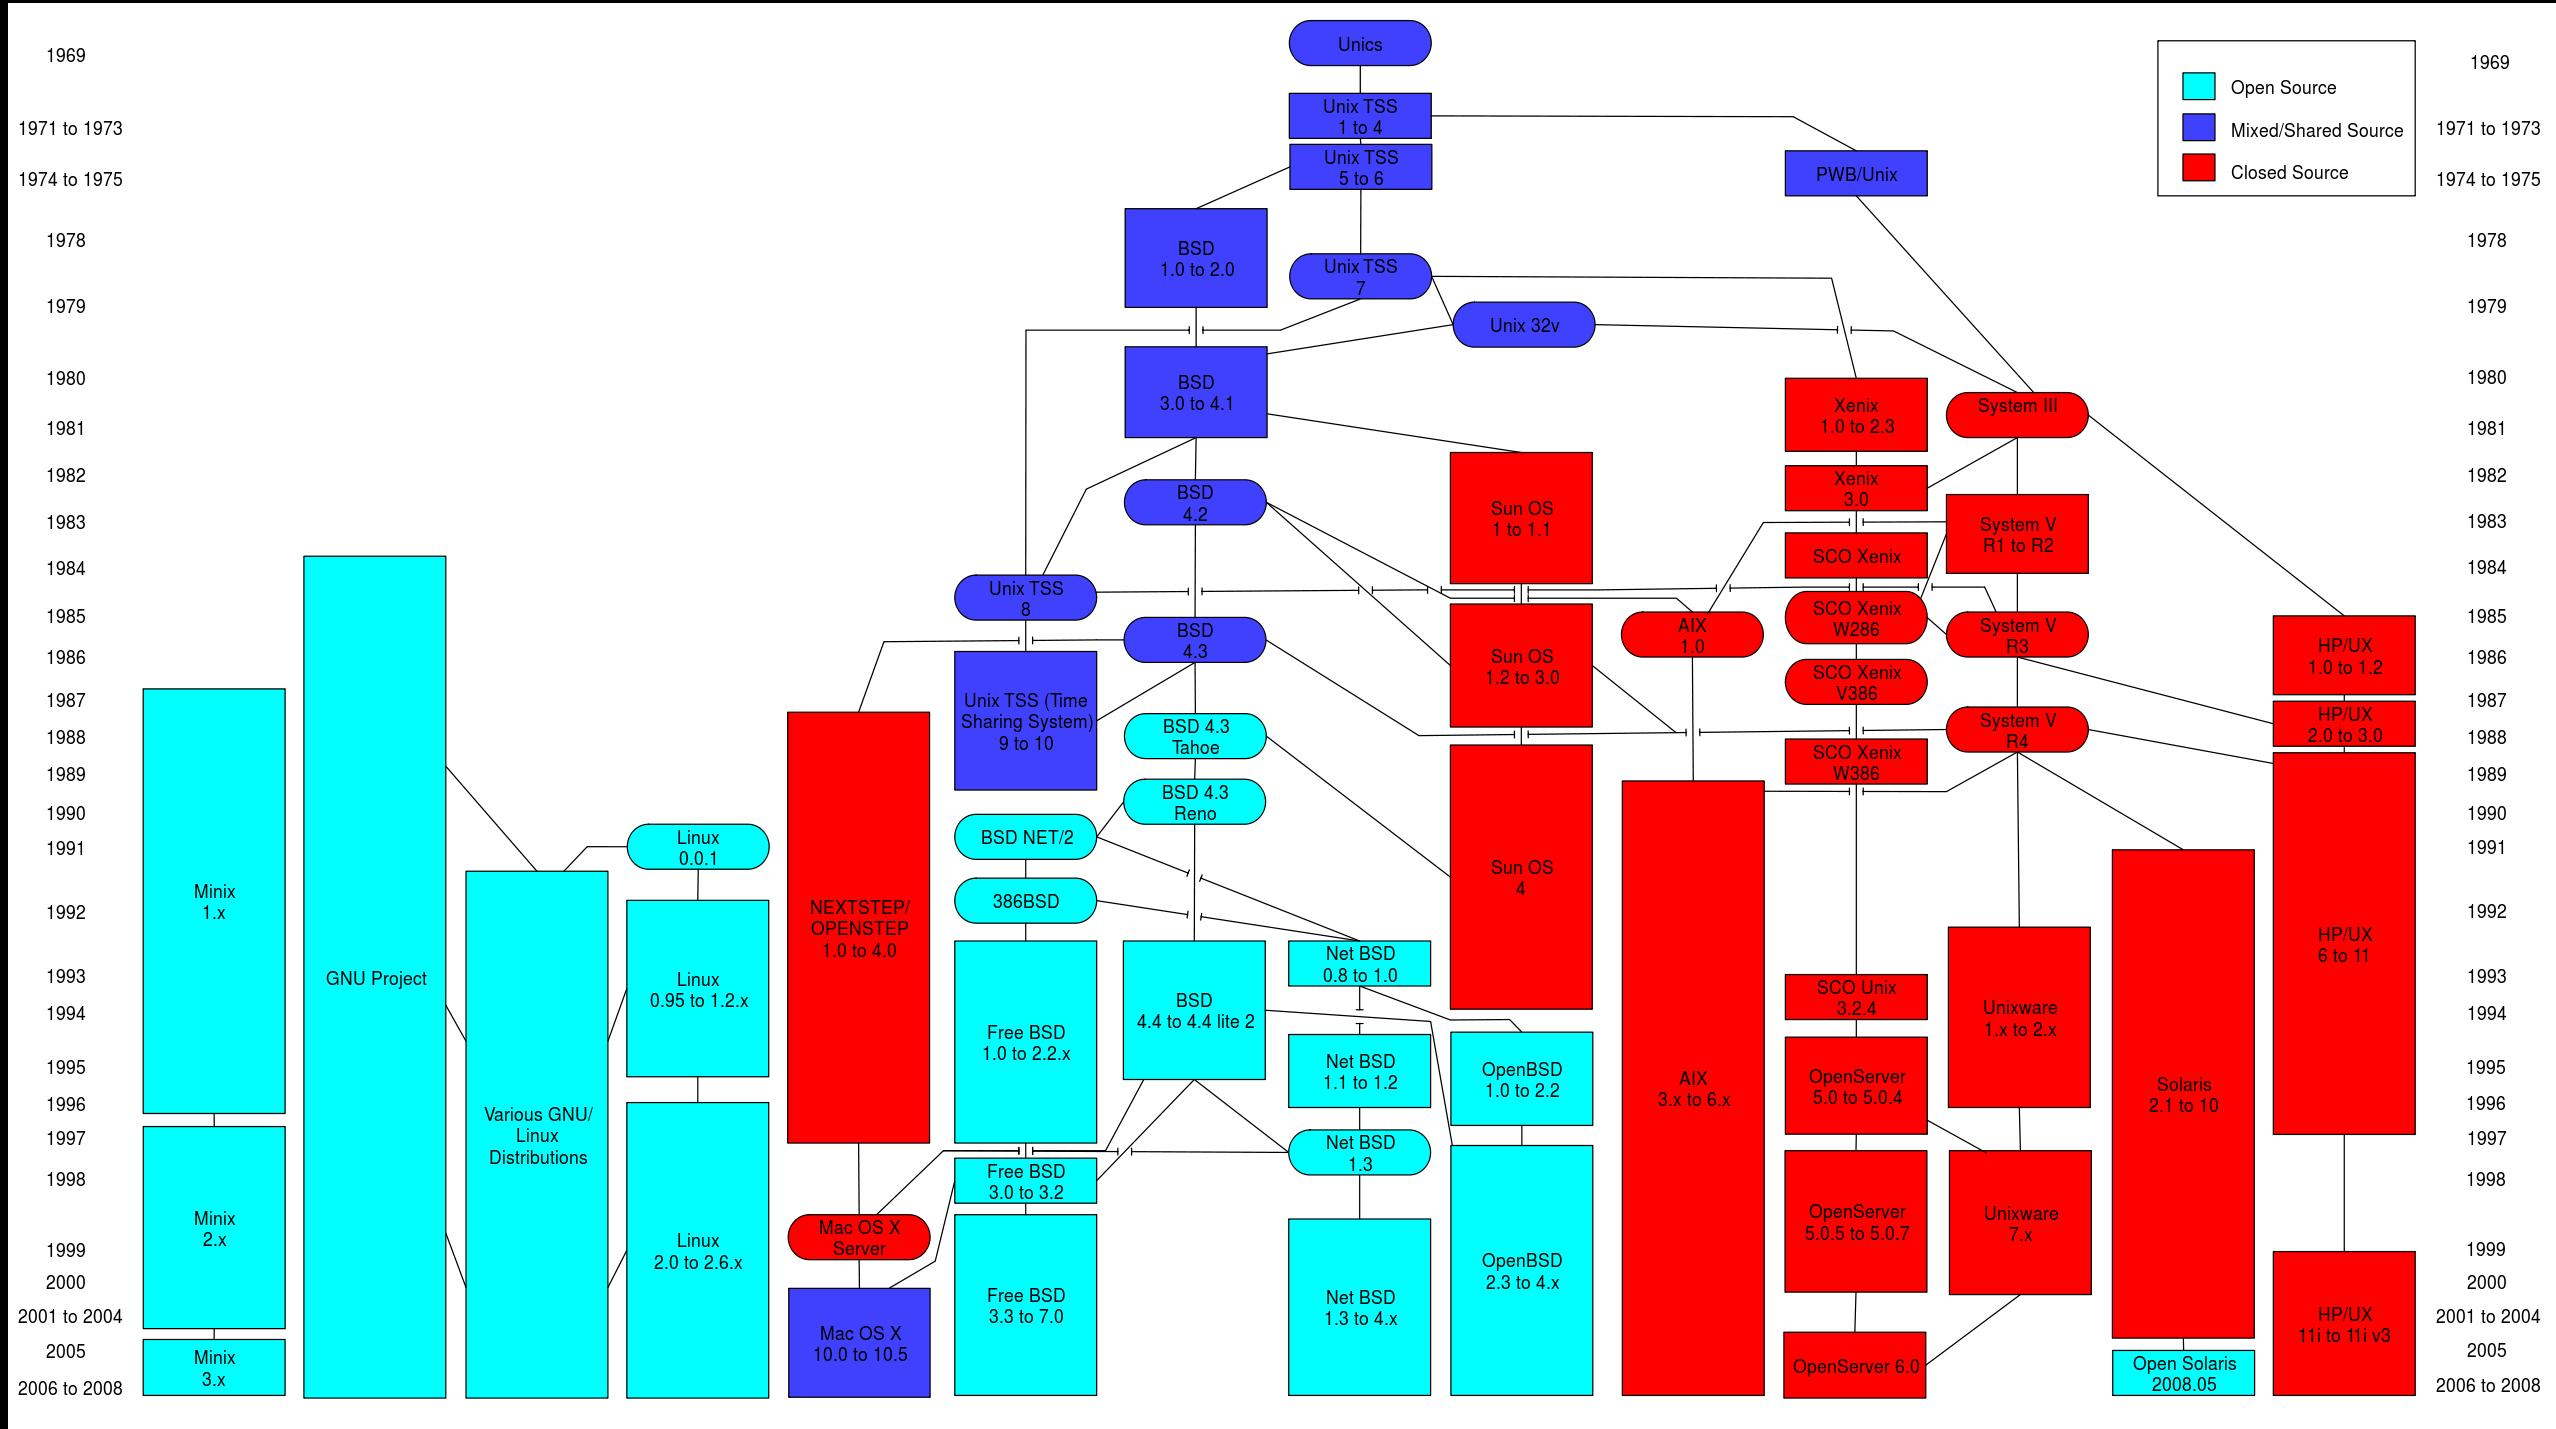
\includegraphics[height=1.90in]{figs/Unix_history-simple.jpg}
  \caption{{\footnotesize Historia de Unix.}}
\end{center}
\end{figure}


\end{frame}



%%%%%%%%%%%%%%%%%%%%%%%%%%%%%%%%%%%%%%%%%%%%%%%%%%%%%%%%%%%%%%%%%%%%%%%


\begin{frame}
\frametitle{Años setenta: Nacen los PCs}

\begin{itemize}

\item El primer computador personal (Altair 8800) sale al mercado en 1975 como ``kit''. 
\item Se les llamaba Microordenadores. Su lenguaje era el BASIC.
\item Atrajo a otra nueva generación de jóvenes hackers libertarios: ``computers for the people''.
\item Nace una industria: Apple se fundó en 1977. Microsoft en 1975 (para vender intérpretes de Basic a los usuarios de Altair). 
\item ``Carta abierta a los aficionados''
\item La gran industria lo ignora hasta muy tarde: IBM lanza su PC en 1981.

\end{itemize}

\end{frame}


%%%%%%%%%%%%%%%%%%%%%%%%%%%%%%%%%%%%%%%%%%%%%%%%%%%%%%%%%%%%%%%%%%%%%%%

\begin{frame}
\frametitle{La revolución de los microordenadores}

\begin{figure}[h]

\begin{center}
  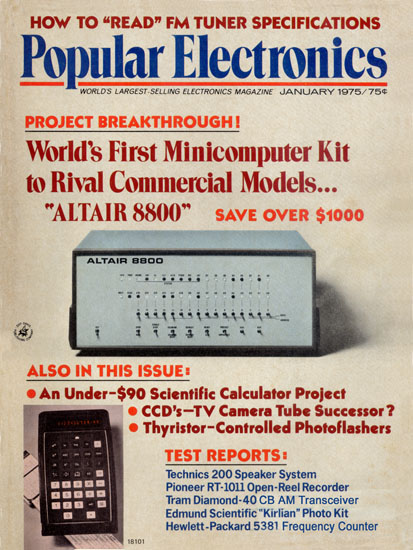
\includegraphics[height=1.80in]{figs/Popular_Electronics_Cover_Jan_1975.jpg}
  \caption{{\footnotesize Portada de \textit{Popular Electronics}, enero de 1975.}}
\end{center}
\end{figure}


\end{frame}

%%%%%%%%%%%%%%%%%%%%%%%%%%%%%%%%%%%%%%%%%%%%%%%%%%%%%%%%%%%%%%%%%%%%%%%

\begin{frame}
\frametitle{La revolución de los microordenadores}


\begin{figure}[h]

\begin{center}
  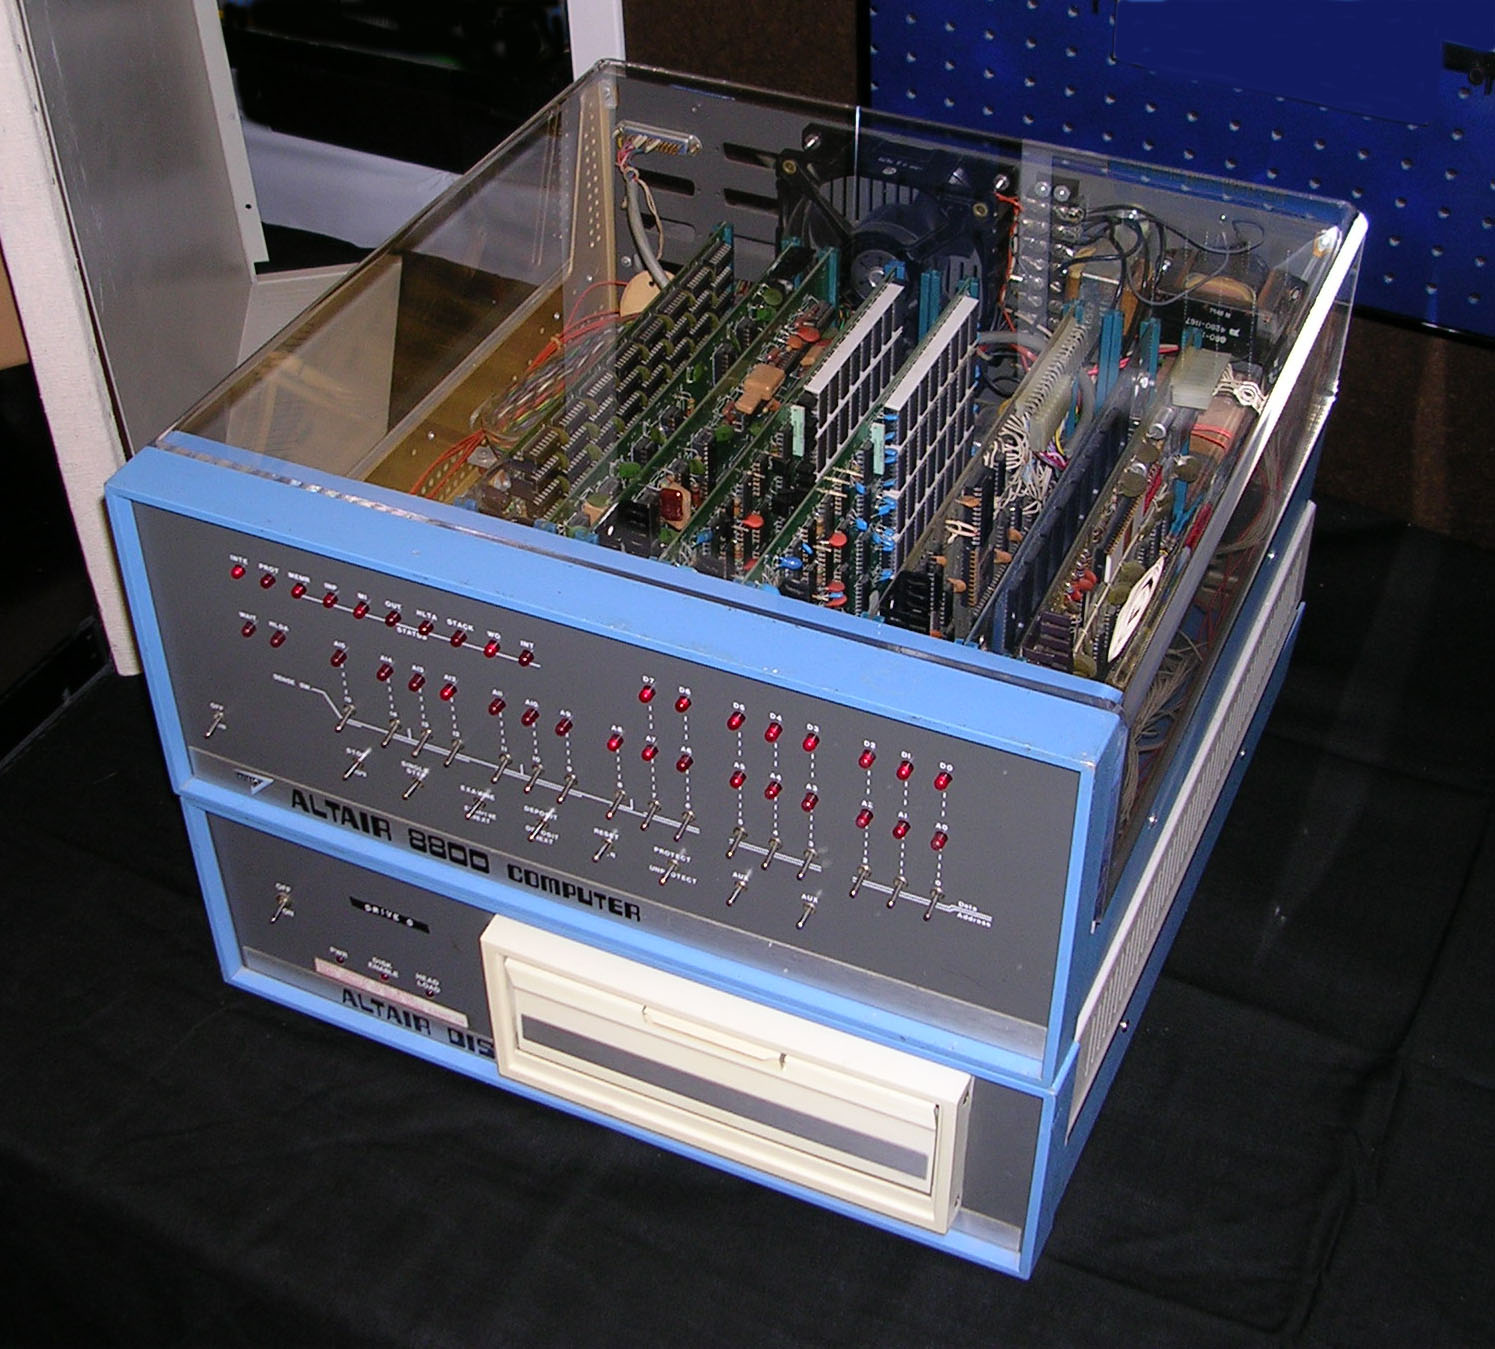
\includegraphics[height=1.80in]{figs/Altair_8800_Computer.jpg}
  \caption{{\footnotesize El MIPS Altair 8800 con disquetera de 8''.}}
\end{center}
\end{figure}


\end{frame}




%%%%%%%%%%%%%%%%%%%%%%%%%%%%%%%%%%%%%%%%%%%%%%%%%%%%%%%%%%%%%%%%%%%%%%%


\begin{frame}
\frametitle{Resumen: Los años setenta y la cultura hacker}

Confluyen tres grandes subculturas hacker a finales de los setenta, en torno a tecnologías muy dispares:

\begin{itemize}

\item \alert{La cultura de las PDP-10 y ARPANET}, ligada a TOPS-10, a LISP (SO del PDP-10), Macro (su lenguaje ensamblador), a ITS, al MIT y al SAIL (IA Lab de Stanford); 
\item \alert{Las gentes de Unix y C} con sus PDP-11, sus VAXen y sus conexiones telefónicas rudimentarias (UUCP). Berkeley y Bell Labs.
\item \alert{Aficionados de los primeros microordenadores}, decididos a acercar el potencial de las computadoras ``al pueblo''. \textit{Popular Electronics}, Altair, Basic, Apple\dots

\end{itemize}

\end{frame}

%%%%%%%%%%%%%%%%%%%%%%%%%%%%%%%%%%%%%%%%%%%%%%%%%%%%%%%%%%%%%%%%%%%%%%%

\begin{frame}

\begin{center}
\huge{Movimiento contemporáneo del software libre}
\end{center}

\end{frame}



%%%%%%%%%%%%%%%%%%%%%%%%%%%%%%%%%%%%%%%%%%%%%%%%%%%%%%%%%%%%%%%%%%%%%%%


\begin{frame}
\frametitle{Años ochenta: El fin de los viejos tiempos}

\begin{itemize}

\item 1983: DEC cancela la línea PDP-10. ITS ya no tiene futuro (no era portable). 
\item {Se extienden los acuerdos de no-divulgación}
\item {Comienza a despegar la gran industria del software privativo, basada en el
secreto (binarios), en la venta de licencias y en la privatización de los fuentes.}
\item Unix e Internet: choca el modelo privativo (AT\&T) contra el modelo abierto (BSD). 

\end{itemize}

\end{frame}


%%%%%%%%%%%%%%%%%%%%%%%%%%%%%%%%%%%%%%%%%%%%%%%%%%%%%%%%%%%%%%%%%%%%%%
%%%%%%%%%%%%%%%%%%%%%%%%%%%%%%%%%%%%%%%%%%%%%%%%%%%%%%%%%%%%%%%%%%%%%%

\begin{frame}
\frametitle{Declina la ética hacker}

Stephen Levy, en \textit{Hackers: Heroes of the Computer Revolution} (1984), acuña la expresión ``ética hacker'' de forma retrospectiva:

\begin{enumerate}
\item Acceso ilimitado a los ordenadores y a todo aquello que puede enseñarte algo.
\item Toda la información debe ser libre
\item Es necesario promover la descentralización
\item Los hackers no deben ser juzgados por sus títulos académicos, su edad o posición.
\item Se puede crear belleza con una computadora.
\item Los ordenadores pueden cambiar la vida a mejor.
\end{enumerate}

\pause

\begin{center}
\alert{El software libre es el heredero directo de estos principios.}
\end{center}

\end{frame}

%%%%%%%%%%%%%%%%%%%%%%%%%%%%%%%%%%%%%%%%%%%%%%%%%%%%%%%%%%%%%%%%%%%%%%

\begin{frame}
\frametitle{Años ochenta: El Proyecto GNU}


\begin{itemize}
\item Stallman abandona el MIT en 1984 para poder dedicarse al Proyecto GNU (GNU's Not UNIX!). 
\item 1985: Stallman publica el Manifiesto GNU: sienta los fundamentos éticos del software libre
\item Meta: construir un sistema completo libre, alternativo a Unix.
\item Crea la infraestructura básica: editor (emacs), compilador (gcc), depurador (gdb), gmake... 
\item Crea la Fundación de Software Libre (1985) para apoyar el Proyecto GNU.
\item Fundamentos legales: la GPL (1989)
\item Trabajo muy estructurado y con metas claras.
\item A principios de los 1990 GNU tenía su sistema casi completo, faltaba el núcleo.

\end{itemize}

\end{frame}


%%%%%%%%%%%%%%%%%%%%%%%%%%%%%%%%%%%%%%%%%%%%%%%%%%%%%%%%%%%%%%%%%%%%%%

\begin{frame}
\frametitle{Final de los 1980, primeros 1990}

CSRG de Berkeley:
\begin{itemize}
\item Liberaron la parte de UNIX (implementación de TCP/IP) que desarrollaron ellos, no AT\&T (Net/1, 1989)
\item Reescribieron el código del UNIX original que no era suyo y liberaron el código (Net/2, 1991)
\item Los hermanos Jolitz portan el código a i386 como 386BSD, liberado por Internet con licencia BSD.
\item Rápidamente: sistemas completos, similares a SunOS en funcionalidad.
\item Importancia de X Window (MIT): cientos de individuos de decenas de empresas colaborando.

\end{itemize}

\end{frame}


%%%%%%%%%%%%%%%%%%%%%%%%%%%%%%%%%%%%%%%%%%%%%%%%%%%%%%%%%%%%%%%%%%%%%%

\begin{frame}
\frametitle{El juicio AT\&T vs BSD}

\begin{itemize}
\item USL (AT\&T) denuncia a la Universidad de Berkeley (1992) por explotar Unix.
\item Berkeley contraataca denunciando a AT\&T por incumplir la licencia BSD (la menos restrictiva del mundo).
\item Berkeley gana el litigio, USL es vendido a Novell y llegan a un acuerdo en 1993.
\item Pero juicio deja exhausto a BSD, supone un retraso de dos años en un momento crítico...
\item Otro proyecto sin problemas legales empieza a adquirir masa... el núcleo Linux.
\item Tras el juicio, se libera una última versión completa de Unix BSD y el CSRG de Berkeley desaparece.

\end{itemize}

\end{frame}

%%%%%%%%%%%%%%%%%%%%%%%%%%%%%%%%%%%%%%%%%%%%%%%%%%%%%%%%%%%%%%%%%%%%%%

\begin{frame}
\frametitle{La herencia de BSD}

\begin{itemize}
\item Desde la distribución de 386BSD el desarrollo es rápido y se consigue un sistema estable.
\item Las distribuciones NetBSD, FreeBSD y OpenBSD surgen a partir de la adaptación original de 386BSD.
\item Modelo catedral, en paralelo al desarrollo de Linux.
\end{itemize}

\end{frame}



%%%%%%%%%%%%%%%%%%%%%%%%%%%%%%%%%%%%%%%%%%%%%%%%%%%%%%%%%%%%%%%%%%%%%%

\begin{frame}
\frametitle{Los años noventa: El nacimiento de Linux}


\begin{itemize}

\item {Linux es un kernel}
\item {Lo inicia Linus Torvalds, en 1991, y \textit{just for fun}}
\item {Existían ya sistema operativos libres casi completos (GNU y Unix BSD)}
\item Desde que liberó la primera versión (0.01) se van uniendo cientos de desarrolladores
\item Se adopta la licencia GPL
\item Marzo 1994: versión 1.0

\end{itemize}

\end{frame}

%%%%%%%%%%%%%%%%%%%%%%%%%%%%%%%%%%%%%%%%%%%%%%%%%%%%%%%%%%%%%%%%%%%%%%

\begin{frame}
\frametitle{Los años noventa: GNU/Linux}


\begin{itemize}

\item Linux es \textit{solo} un kernel: necesita algo más para funcionar.
\item Al proyecto GNU le falta un núcleo en 1990.
\item Desarrollo del proyecto Hurd, arquitectura de microkernel (Mach): sin resultados
\item Se adopta \textit{temporalmente} como núcleo para GNU
\item Proliferan las distribuciones GNU/Linux: Slackware, Debian, Red Hat, SuSE, Gentoo, etc.

\end{itemize}

\end{frame}

%%%%%%%%%%%%%%%%%%%%%%%%%%%%%%%%%%%%%%%%%%%%%%%%%%%%%%%%%%%%%%%%%%%%%%

\begin{frame}
\frametitle{Los años noventa: el modelo bazar}


\begin{itemize}

\item ``La ventaja más importante de Linux no fue de carácter técnico, sino sociológico'' (ESR -- CATB).
\item {La principal aportación de Linu[xs]: su modelo de desarrollo, el llamado ``modelo bazar''}
\item Gran número de voluntarios coordinados a través de Internet. 
\item La calidad se mantenía, no con estándares rígidos o autocracia, sino publicando cada semana y obteniendo el \textit{feedback} de cientos de usuarios pocos días.
\item ``\textit{Release Early, Release Often} (and listen to your customers)'': propicia selección darwiniana rápida sobre las mutaciones presentadas por los desarrolladores. 
\item Para sorpresa de casi todo el mundo, esto funcionó bastante bien. 
\end{itemize}

\end{frame}



%%%%%%%%%%%%%%%%%%%%%%%%%%%%%%%%%%%%%%%%%%%%%%%%%%%%%%%%%%%%%%%%%%%%%%

\begin{frame}
\frametitle{Finales de los 1990}

\begin{itemize}
\item Netscape anuncia la liberación del código de su navegador: 
\item ``La catedral y el bazar''.
\item Cada vez más cerca del usuario estándar: KDE, GNOME.
\item GNU/Linux penetra en Universidades (y en casa de los
estudiantes).
\item La mejor opción es libre en muchos ámbitos (Apache, infraestructura de Internet, XFree, GCC, Gnat).
\item Empresas como RedHat consiguen capital-riesgo. Nasdaq: IPOs de récord.
\item La prensa comienza a atender al software libre: compite con Windows NT.
\item Grandes empresas tecnológicas invierten en Software Libre: HP, IBM, Sun, Google, Yahoo!...
\end{itemize}

\end{frame}


%%%%%%%%%%%%%%%%%%%%%%%%%%%%%%%%%%%%%%%%%%%%%%%%%%%%%%%%%%%%%%%%%%%%%%

\begin{frame}
\frametitle{Principios de los 2000: Madurando poco a poco}

\begin{itemize}
\item El software libre empieza a estar listo para el escritorio (GNOME 2.x, KDE 3.x, OpenOffice), y es simple de instalar por el usuario final.
\item El software libre se incorpora a la estrategia de grandes empresas (IBM, HP, Sun)
\item Otras (como Microsoft) prefieren una estrategia de enfrentamiento parcial (FUD).
\item Difcultades financieras como resultado de la crisis de las puntocom
\item Comienza la penetración en Administraciones públicas y grandes empresas
\item Aumento grande del número de desarrolladores, de la cantidad de software libre disponible, etc.
\end{itemize}

\end{frame}

%%%%%%%%%%%%%%%%%%%%%%%%%%%%%%%%%%%%%%%%%%%%%%%%%%%%%%%%%%%%%%%%%%%%%%

\begin{frame}
\frametitle{Principios de los 2000: Madurando poco a poco}


Productos con éxito:
\begin{itemize}
\item Servidores: Apache, Postfix, Tomcat, Proftpd...
\item Navegadores: primero Mozilla, luego Firefox...
\item Correo: Thunderbird, Evolution, Kmail...
\item Ofimática: LibreOffice, Koffice, AbiWord...
\item Escritorio: KDE, Gnome, Compiz/Beryl...
\item Sistemas Operativos: Sun libera Solaris (2005) y todas sus tecnologías punteras (ZFS, DTrace, etc.).
\item Formatos abiertos: ODF (ISO/IEC 26300), OGG...
\end{itemize}

\end{frame}
 

%%%%%%%%%%%%%%%%%%%%%%%%%%%%%%%%%%%%%%%%%%%%%%%%%%%%%%%%%%%%%%%%%%%%%%

\begin{frame}
\frametitle{Principios de los 2000 (2)}

\begin{itemize}
\item Nuevas disciplinas estudian el software libre: comenzamos, poco a poco, a entender cómo funciona
\item Comienzan a verse efectos de la ``deslocalización'' del desarrollo de software libre: países periféricos hacen cosas
interesantes.
\item Ciertos mercados, ciertos sectores, ya consideran al software libre como una opción natural
\item El entorno legal va cambiando de forma ambivalente: ¿se convertirá en hostil para el software libre?
\end{itemize}

\end{frame}

%%%%%%%%%%%%%%%%%%%%%%%%%%%%%%%%%%%%%%%%%%%%%%%%%%%%%%%%%%%%%%%%%%%%%%

\begin{frame}
\frametitle{Actualidad (finales de los 2000)}

\begin{itemize}
\item Software libre es estratégico para muchas empresas (ej: Google)
\item Conjuntos de aplicaciones muy completos para muchos entornos
\item Empresas probando nuevos modelos de colaboración (ej: ObjectWeb, Morfeo)
\item Software libre como propuesta para dominar mercados (ej: Android, Symbian, Maemo en móviles)
\item Nuevos modelos de negocio, modelos para nuevos negocios
\item Software libre parte del análisis de competencia en sectores (ej: MySQL en la compra de Sun por Oracle)
\item Software libre se analiza en las Escuelas de Negocios.
\item El software libre se va convirtiendo en algo ``normal''.
\end{itemize}

\end{frame}

%%%%%%%%%%%%%%%%%%%%%%%%%%%%%%%%%%%%%%%%%%%%%%%%%%%%%%%%%%%%%%%%%%%%%%

\begin{frame}
\frametitle{El futuro: ¿una carrera de obstáculos?}

La evolución futura del software libre se encuentra con varios
obstáculos:

\begin{itemize}
\item Técnicas FUD (miedo, incertidumbre, duda): hasta ahora han mostrado no ser muy problemáticas.
\item Disolución: confusión (llamar libre a lo que no lo es), división de la comunidad, pérdida de las
ventajas del modelo...
\item Desconocimiento (pérdida de visión): ¿por qué es interesante el software libre?
\item Impedimentos legales y tecnológicos: patentes de software, mecanismos de
control de acceso a la información, leyes contrarias (anti-elusión), etc.
\item ¿Cómo es de sostenible el desarrollo de software libre?
\end{itemize}

\end{frame}


%%==================================================================
%%---------------------------------------------------------------


\end{document}

%%==================================================================
%%---------------------------------------------------------------

